<tipo = seleccion unica, orden = aleatorio>

<pregunta>
El exterior de un cubo está pintado con cuadrados blancos y negros como si se hubiera construido con cuatro cubos blancos y cuatro cubos negros. ¿Cuál de las siguientes figuras corresponde al esquema correcto para la construcción de dicho cubo? \\[1ex]
\centerline{
	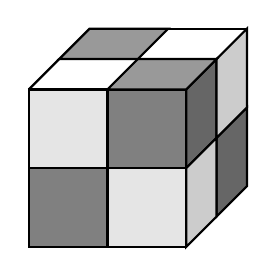
\begin{tikzpicture}[thick]
		\filldraw[fill=black!60] (2,0,0) -- (2,1,0) -- (2,1,1) -- (2,0,1) -- cycle;
		\filldraw[fill=black!60] (2,2,2) -- (2,1,2) -- (2,1,1) -- (2,2,1) -- cycle;
		\filldraw[fill=black!20] (2,2,1) -- (2,1,1) -- (2,1,0) -- (2,2,0) -- cycle;
		\filldraw[fill=black!20] (2,0,1) -- (2,1,1) -- (2,1,2) -- (2,0,2) -- cycle;
		\filldraw[fill=black!50] (0,0,2) rectangle (1,1,2);
		\filldraw[fill=black!50] (1,1,2) rectangle (2,2,2);
		\filldraw[fill=black!10] (1,0,2) rectangle (2,1,2);
		\filldraw[fill=black!10] (0,1,2) rectangle (1,2,2);
		\filldraw[fill=black!40] (1,2,2) -- (1,2,1) -- (2,2,1) -- (2,2,2) -- cycle;
		\filldraw[fill=black!40] (0,2,1) -- (0,2,0) -- (1,2,0) -- (1,2,1) -- cycle;
		\draw (0,2,2) -- (0,2,1);
		\draw (1,2,0) -- (2,2,0);
  \end{tikzpicture}}
\bigskip

<item>
\raisebox{-3em}{
	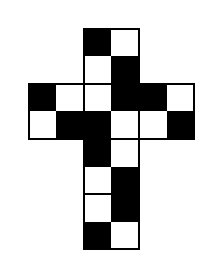
\begin{tikzpicture}[thick,scale=0.7]
		\fill (1,0) rectangle (1.5,0.5);
		\fill (1,1.5) rectangle (1.5,2);
		\fill (1.5,0.5) rectangle (2,1.5);
		\fill (0,2.5) rectangle (0.5,3);
		\fill (0.5,2) rectangle (1.5,2.5);
		\fill (1.5,2.5) rectangle (2.5,3);
		\fill (2.5,2) rectangle (3,2.5);
		\fill (1,3.5) rectangle (1.5,4);
		\fill (1.5,3) rectangle (2,3.5);
		\draw (1,0) rectangle (2,4);
		\draw (0,2) rectangle (3,3);
		\draw (1,1) -- (2,1);
  \end{tikzpicture}}
\bigskip

<item>
\raisebox{-3em}{
	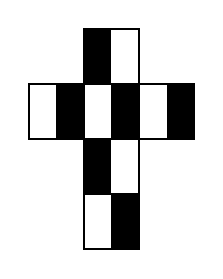
\begin{tikzpicture}[thick,scale=0.7]
		\fill (0.5,2) rectangle (1,3);
		\fill (1.5,2) rectangle (2,3);
		\fill (2.5,2) rectangle (3,3);
		\fill (1.5,0) rectangle (2,1);
		\fill (1,1) rectangle (1.5,2);
		\fill (1,3) rectangle (1.5,4);
		\draw (1,0) rectangle (2,4);
		\draw (0,2) rectangle (3,3);
		\draw (1,1) -- (2,1);
	\end{tikzpicture}}
\bigskip

<item>
\raisebox{-3em}{
	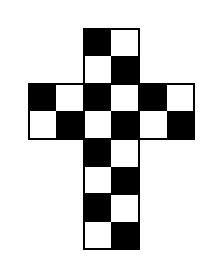
\begin{tikzpicture}[thick,scale=0.7]
		\fill (0,2.5) rectangle (0.5,3);
		\fill (1,2.5) rectangle (1.5,3);
		\fill (2,2.5) rectangle (2.5,3);
		\fill (0.5,2) rectangle (1,2.5);
		\fill (1.5,2) rectangle (2,2.5);
		\fill (2.5,2) rectangle (3,2.5);
		\fill (1,0.5) rectangle (1.5,1);
		\fill (1,1.5) rectangle (1.5,2);
		\fill (1,3.5) rectangle (1.5,4);
		\fill (1.5,0) rectangle (2,0.5);
		\fill (1.5,1) rectangle (2,1.5);
		\fill (1.5,3) rectangle (2,3.5);
		\draw (1,0) rectangle (2,4);
		\draw (0,2) rectangle (3,3);
		\draw (1,1) -- (2,1);
	\end{tikzpicture}}
\bigskip

<item>
\raisebox{-3em}{
	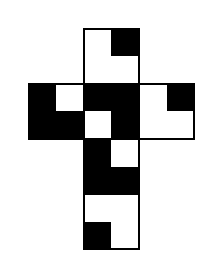
\begin{tikzpicture}[thick,scale=0.7]
		\fill (0,2) rectangle (2,3);
		\fill[white] (0.5,2.5) rectangle (1,3);
		\fill[white] (1,2) rectangle (1.5,2.5);
		\fill (1,0) rectangle (1.5,0.5);
		\fill (1.5,3.5) rectangle (2,4);
		\fill (2.5,2.5) rectangle (3,3);
		\fill (1,1) rectangle (2,2);
		\fill[white] (1.5,1.5) rectangle (2,2);
		\draw (0,2) rectangle (3,3);
		\draw (1,0) rectangle (2,4);
		\draw (1,1) -- (2,1);
	\end{tikzpicture}}
\bigskip

<item>
\raisebox{-3em}{
	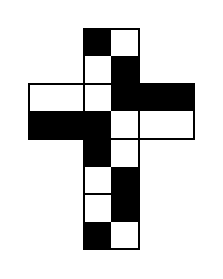
\begin{tikzpicture}[thick,scale=0.7]
		\fill (0,2) rectangle (1.5,2.5);
		\fill (1,1.5) rectangle (1.5,2);
		\fill (1.5,0.5) rectangle (2,1.5);
		\fill (1,0) rectangle (1.5,0.5);
		\fill (1,3.5) rectangle (1.5,4);
		\fill (1.5,2.5) rectangle (2,3.5);
		\fill (2,2.5) rectangle (3,3);
		\draw (1,0) rectangle (2,4);
		\draw (0,2) rectangle (3,3);
		\draw (1,1) -- (2,1);
	\end{tikzpicture}}
\bigskip

